\documentclass[a4paper,12pt,twoside]{memoir}

% Castellano
\usepackage[spanish,es-tabla]{babel}
\selectlanguage{spanish}
\usepackage[utf8]{inputenc}
\usepackage[T1]{fontenc}
\usepackage{lmodern} % Scalable font
\usepackage{microtype}
\usepackage{placeins}

\RequirePackage{booktabs}
\RequirePackage[table]{xcolor}
\RequirePackage{xtab}
\RequirePackage{multirow}

% Links
\PassOptionsToPackage{hyphens}{url}\usepackage[colorlinks]{hyperref}
\hypersetup{
	allcolors = {red}
}

% Ecuaciones
\usepackage{amsmath}

% Rutas de fichero / paquete
\newcommand{\ruta}[1]{{\sffamily #1}}

% Párrafos
\nonzeroparskip

% Huérfanas y viudas
\widowpenalty100000
\clubpenalty100000

% Imágenes

% Comando para insertar una imagen en un lugar concreto.
% Los parámetros son:
% 1 --> Ruta absoluta/relativa de la figura
% 2 --> Texto a pie de figura
% 3 --> Tamaño en tanto por uno relativo al ancho de página
\usepackage{graphicx}
\newcommand{\imagen}[3]{
	\begin{figure}[!h]
		\centering
		\includegraphics[width=0.9\textwidth]{#1}
		\caption{#2}\label{fig:#1}
	\end{figure}
	\FloatBarrier
}

% Comando para insertar una imagen sin posición.
% Los parámetros son:
% 1 --> Ruta absoluta/relativa de la figura
% 2 --> Texto a pie de figura
% 3 --> Tamaño en tanto por uno relativo al ancho de página
\newcommand{\imagenflotante}[3]{
	\begin{figure}
		\centering
		\includegraphics[width=#3\textwidth]{#1}
		\caption{#2}\label{fig:#1}
	\end{figure}
}

% El comando \figura nos permite insertar figuras comodamente, y utilizando
% siempre el mismo formato. Los parametros son:
% 1 --> Porcentaje del ancho de página que ocupará la figura (de 0 a 1)
% 2 --> Fichero de la imagen
% 3 --> Texto a pie de imagen
% 4 --> Etiqueta (label) para referencias
% 5 --> Opciones que queramos pasarle al \includegraphics
% 6 --> Opciones de posicionamiento a pasarle a \begin{figure}
\newcommand{\figuraConPosicion}[6]{%
  \setlength{\anchoFloat}{#1\textwidth}%
  \addtolength{\anchoFloat}{-4\fboxsep}%
  \setlength{\anchoFigura}{\anchoFloat}%
  \begin{figure}[#6]
    \begin{center}%
      \Ovalbox{%
        \begin{minipage}{\anchoFloat}%
          \begin{center}%
            \includegraphics[width=\anchoFigura,#5]{#2}%
            \caption{#3}%
            \label{#4}%
          \end{center}%
        \end{minipage}
      }%
    \end{center}%
  \end{figure}%
}

%
% Comando para incluir imágenes en formato apaisado (sin marco).
\newcommand{\figuraApaisadaSinMarco}[5]{%
  \begin{figure}%
    \begin{center}%
    \includegraphics[angle=90,height=#1\textheight,#5]{#2}%
    \caption{#3}%
    \label{#4}%
    \end{center}%
  \end{figure}%
}
% Para las tablas
\newcommand{\otoprule}{\midrule [\heavyrulewidth]}
%
% Nuevo comando para tablas pequeñas (menos de una página).
\newcommand{\tablaSmall}[5]{%
 \begin{table}
  \begin{center}
   \rowcolors {2}{gray!35}{}
   \begin{tabular}{#2}
    \toprule
    #4
    \otoprule
    #5
    \bottomrule
   \end{tabular}
   \caption{#1}
   \label{tabla:#3}
  \end{center}
 \end{table}
}

%
% Nuevo comando para tablas pequeñas (menos de una página).
\newcommand{\tablaSmallSinColores}[5]{%
 \begin{table}[H]
  \begin{center}
   \begin{tabular}{#2}
    \toprule
    #4
    \otoprule
    #5
    \bottomrule
   \end{tabular}
   \caption{#1}
   \label{tabla:#3}
  \end{center}
 \end{table}
}

\newcommand{\tablaApaisadaSmall}[5]{%
\begin{landscape}
  \begin{table}
   \begin{center}
    \rowcolors {2}{gray!35}{}
    \begin{tabular}{#2}
     \toprule
     #4
     \otoprule
     #5
     \bottomrule
    \end{tabular}
    \caption{#1}
    \label{tabla:#3}
   \end{center}
  \end{table}
\end{landscape}
}

%
% Nuevo comando para tablas grandes con cabecera y filas alternas coloreadas en gris.
\newcommand{\tabla}[6]{%
  \begin{center}
    \tablefirsthead{
      \toprule
      #5
      \otoprule
    }
    \tablehead{
      \multicolumn{#3}{l}{\small\sl continúa desde la página anterior}\\
      \toprule
      #5
      \otoprule
    }
    \tabletail{
      \hline
      \multicolumn{#3}{r}{\small\sl continúa en la página siguiente}\\
    }
    \tablelasttail{
      \hline
    }
    \bottomcaption{#1}
    \rowcolors {2}{gray!35}{}
    \begin{xtabular}{#2}
      #6
      \bottomrule
    \end{xtabular}
    \label{tabla:#4}
  \end{center}
}

%
% Nuevo comando para tablas grandes con cabecera.
\newcommand{\tablaSinColores}[6]{%
  \begin{center}
    \tablefirsthead{
      \toprule
      #5
      \otoprule
    }
    \tablehead{
      \multicolumn{#3}{l}{\small\sl continúa desde la página anterior}\\
      \toprule
      #5
      \otoprule
    }
    \tabletail{
      \hline
      \multicolumn{#3}{r}{\small\sl continúa en la página siguiente}\\
    }
    \tablelasttail{
      \hline
    }
    \bottomcaption{#1}
    \begin{xtabular}{#2}
      #6
      \bottomrule
    \end{xtabular}
    \label{tabla:#4}
  \end{center}
}

%
% Nuevo comando para tablas grandes sin cabecera.
\newcommand{\tablaSinCabecera}[5]{%
  \begin{center}
    \tablefirsthead{
      \toprule
    }
    \tablehead{
      \multicolumn{#3}{l}{\small\sl continúa desde la página anterior}\\
      \hline
    }
    \tabletail{
      \hline
      \multicolumn{#3}{r}{\small\sl continúa en la página siguiente}\\
    }
    \tablelasttail{
      \hline
    }
    \bottomcaption{#1}
  \begin{xtabular}{#2}
    #5
   \bottomrule
  \end{xtabular}
  \label{tabla:#4}
  \end{center}
}



\definecolor{cgoLight}{HTML}{EEEEEE}
\definecolor{cgoExtralight}{HTML}{FFFFFF}

%
% Nuevo comando para tablas grandes sin cabecera.
\newcommand{\tablaSinCabeceraConBandas}[5]{%
  \begin{center}
    \tablefirsthead{
      \toprule
    }
    \tablehead{
      \multicolumn{#3}{l}{\small\sl continúa desde la página anterior}\\
      \hline
    }
    \tabletail{
      \hline
      \multicolumn{#3}{r}{\small\sl continúa en la página siguiente}\\
    }
    \tablelasttail{
      \hline
    }
    \bottomcaption{#1}
    \rowcolors[]{1}{cgoExtralight}{cgoLight}

  \begin{xtabular}{#2}
    #5
   \bottomrule
  \end{xtabular}
  \label{tabla:#4}
  \end{center}
}



\graphicspath{ {./img/} }

% Capítulos
\chapterstyle{bianchi}
\newcommand{\capitulo}[2]{
	\setcounter{chapter}{#1}
	\setcounter{section}{0}
	\setcounter{figure}{0}
	\setcounter{table}{0}
	\chapter*{#2}
	\addcontentsline{toc}{chapter}{#2}
	\markboth{#2}{#2}
}

% Apéndices
\renewcommand{\appendixname}{Apéndice}
\renewcommand*\cftappendixname{\appendixname}

\newcommand{\apendice}[1]{
	%\renewcommand{\thechapter}{A}
	\chapter{#1}
}

\renewcommand*\cftappendixname{\appendixname\ }

% Formato de portada
\makeatletter
\usepackage{xcolor}
\newcommand{\tutor}[1]{\def\@tutor{#1}}
\newcommand{\course}[1]{\def\@course{#1}}
\definecolor{cpardoBox}{HTML}{E6E6FF}
\def\maketitle{
  \null
  \thispagestyle{empty}
  % Cabecera ----------------
\noindent
\includegraphics[width=\textwidth]{cabecera}\vspace{1cm}%
  \vfill
  % Título proyecto y escudo informática ----------------
  \colorbox{cpardoBox}{%
    \begin{minipage}{.8\textwidth}
      \vspace{.5cm}\Large
      \begin{center}
      \textbf{TFG del Grado en Ingeniería Informática}\vspace{.6cm}\\
      \textbf{\LARGE\@title{}}
      \end{center}
      \vspace{.2cm}
    \end{minipage}

  }%
  \hfill\begin{minipage}{.20\textwidth}
    
\includegraphics[width=\textwidth]{escudoInfor}
  \end{minipage}
  \vfill
  % Datos de alumno, curso y tutores ------------------
  \begin{center}%
  {%
    \noindent\LARGE
    Presentado por \@author{}\\ 
    en Universidad de Burgos --- \@date{}\\
    Tutor: \@tutor{}\\
  }%
  \end{center}%
  \null
  \cleardoublepage
  }
\makeatother

\newcommand{\nombre}{Alex Tomé Aguiar} %%% cambio de comando

% Datos de portada
\title{CSACVM - Gestor de currículos para CSA}
\author{Alex Tomé Aguiar}
\tutor{Carlos Pardo Aguilar y Sandra Rodríguez Arribas}
\date{\today}

\begin{document}

\maketitle


\newpage\null\thispagestyle{empty}\newpage\newpage


%%%%%%%%%%%%%%%%%%%%%%%%%%%%%%%%%%%%%%%%%%%%%%%%%%%%%%%%%%%%%%%%%%%%%%%%%%%%%%%%%%%%%%%%
\thispagestyle{empty}


\noindent
\includegraphics[width=\textwidth]{cabecera}\vspace{1cm}

\noindent D. Carlos Pardo Aguilar y Dña. Sandra Rodríguez Arribas, profesores del departamento de Ingeniería Informática, área de Lenguajes y Sistemas Informáticos.

\noindent Exponen:

\noindent Que el alumno D. \nombre, con DNI 71307554X, ha realizado el Trabajo final de Grado en Ingeniería Informática titulado ``CSACVM - Gestión de Currículum Vitae para CSA''. 

\noindent Y que dicho trabajo ha sido realizado por el alumno bajo la dirección del que suscribe, en virtud de lo cual se autoriza su presentación y defensa.

\begin{center} %\large
En Burgos, {\large \today}
\end{center}

\vfill\vfill\vfill

% Author and supervisor
\begin{minipage}{0.45\textwidth}
\begin{flushleft} %\large
Vº. Bº. del Tutor:\\[2cm]
Dña. Sandra Rodríguez Arribas
\end{flushleft}
\end{minipage}
\hfill
\begin{minipage}{0.45\textwidth}
\begin{flushleft} %\large
Vº. Bº. del co-tutor:\\[2cm]
D. Carlos Pardo Aguilar
\end{flushleft}
\end{minipage}
\hfill

\vfill

% para casos con solo un tutor comentar lo anterior
% y descomentar lo siguiente
%Vº. Bº. del Tutor:\\[2cm]
%D. nombre tutor


\newpage\null\thispagestyle{empty}




\frontmatter

% Abstract en castellano
\renewcommand*\abstractname{Resumen}
\begin{abstract}
Cada vez que queremos solicitar un puesto en una empresa, debemos tener siempre actualizado nuestro currículum. Esto puede ser muy molesto en el caso de que se haga a mano, y varias aplicaciones que se pueden encontrar por Internet no resultan del todo cómodas para ellos. 

Desde el punto de vista de la empresa es todavía peor, pues cada currículum tiene un formato y estructura diferentes y es tedioso a la hora de filtrarlos por los trabajadores de la empresa.

Esta aplicación web, CSACVM, ofrece una gestión de currículos para la empresa CSA, de manera que cada currículum es igual en cuanto a formato y estructura. Además de esto, todos los usuarios podrán mantenerlo actualizado y, además, los trabajadores de la empresa podrán acceder y filtrar a través de toda clase de información para facilitar el análisis de estos documentos.
\end{abstract}

\renewcommand*\abstractname{Descriptores}
\begin{abstract}
Aplicación web, ASP.NET Core, Currículum Vitae, base de datos, gestión, documentos, usuarios, empresa.
\end{abstract}

\clearpage

% Abstract en inglés
\renewcommand*\abstractname{Abstract}
\begin{abstract}
Everytime we want to apply for a job, we need to have our Curriculum Vitae updated. This can be annoying at some point if we do this by hand, and some Internet apps may be not convinient or suitable for it. 

Regarding the company's point of view, it is even worse, because every Curriculum Vitae has a different structure and format so it makes it annoying to filter the user information by the company's worker.

This web application, CSACVM, offers a Curriculum Vitae management for the CSA company, in order to make every curriculum as equal as possible in terms of structure and format. Moreover, every user can make them be updated and also, the company's workers will be able to filter and access to every type of information of the curriculum to make it easier for them to analyse the documents.
\end{abstract}

\renewcommand*\abstractname{Keywords}
\begin{abstract}
Web Application, ASP.NET Core, Currículum Vitae, database, management, documents, users, company.
\end{abstract}

\clearpage

% Indices
\tableofcontents

\clearpage

\listoffigures

\clearpage


\mainmatter
\capitulo{1}{Introducción}

En esta parte de la documentación se describirá el contexto de la aplicación en base a qué
problemas existen, cómo surge la idea y cómo se van a solucionar dichos problemas. Asimismo, 
se describe la estructura de la memoria y los elementos que se adjuntan.

\section{Contexto}
Cada vez que queremos solicitar un puesto en una empresa, debemos tener 
siempre actualizado nuestro currículum. Esto puede ser muy molesto en el caso
de que se haga a mano, y varias aplicaciones que se pueden encontrar por Internet 
no resultan del todo cómodas para esto.

Desde el punto de vista de la empresa es todavía peor, pues cada currículum tiene un 
formato y estructura diferentes y es tedioso a la hora de filtrarlos por los trabajadores
de la empresa.

Y esto ya no solo es un problema para los currículos que vienen de nuevos trabajadores,
sino que también lo es para los que llevan un determinado tiempo en la empresa, ya que,
al estar hechos a mano, pueden estar años sin actualizarse.

El principal problema que se aborda en esta aplicación es el resultante de todo lo mencionado
previamente: se necesita un gestor interno que unifique la estructura y el formato
de, no solo los currículos de nuevos trabajadores, sino de aquellos que lleven tiempo
en la empresa y, además, que estos últimos se mantengan actualizados con el tiempo.

\section{Estructura del TFG}

La documentación entregada se divide en dos partes: la memoria y los anexos.
La memoria comprende este documento y tiene la siguiente estructura:

\begin{itemize}
\item
  \textbf{Introducción:} breve descripción del problema a resolver y la
  solución propuesta. Estructura de la memoria y listado de materiales
  adjuntos.
\item
  \textbf{Objetivos del proyecto:} las diferentes metas que se quieren 
  alcanzar a través del proyecto.
\item
  \textbf{Conceptos teóricos:} explicaciones teóricas sobre el funcionamiento de varias
  de las herramientas que se utilizan, como librerías y dependencias.
\item
  \textbf{Técnicas y herramientas:} listado de las diferentes utilidades
  que se usan en el desarrollo del proyecto, tales el como entorno, lenguajes,
  librerías, etc.
\item
  \textbf{Aspectos relevantes del desarrollo:} aspectos a destacar durante el
  desarrollo de la aplicación que puedan tener cierto interés informativo.
\item
  \textbf{Trabajos relacionados:} estudio de otras aplicaciones o herramientas similares
  a la que se presenta y sus diferencias, así como un análisis de necesidad del desarrollo de
  esta aplicación en función de las buscadas.
\item
  \textbf{Conclusiones y líneas de trabajo futuras:} conclusiones que se obtienen
  al finalizar el proyecto y posibles mejoras a futuro.
\end{itemize}

Los anexos, a su vez, tienen la siguiente estructura:
\begin{itemize}
\item
  \textbf{Plan del proyecto:} planificación de las diferentes fases que abarcan 
  el proyecto y estudio de la viabilidad del mismo.
\item
  \textbf{Especificación de requisitos del software:} se describe qué es necesario
  hacer en cuanto a estructura y funcionalidad del proyecto, descripción del problema
  y alcance de los requisitos.
\item
  \textbf{Especificación de diseño:} se describe el diseño de las diferentes partes
  que forman la estructura del proyecto, tales como la base de datos, la arquitectura,
  páginas, etc.
\item
  \textbf{Manual del programador:} manual técnico que recoge aspectos importantes del 
  código del proyecto y de la instalación del servidor.
\item
  \textbf{Manual de usuario:} manual orientado a la guía de la aplicación para los
  usuarios que quieran utilizarla en cuanto a funcionamiento y comprensión de las distintas
  partes de la aplicación.
\end{itemize}

\section{Otros materiales}
Junto a la memoria y los anexos, también se adjuntan otros materiales. En este caso 
se entrega el más importante para las pruebas del proyecto, que es la máquina virtual.

La máquina virtual se entrega en forma de ``.ova'' y tiene las siguientes partes:

\begin{itemize}
\item
	SQL Server con la base de datos activa.
\item
	IIS Express configurado con la aplicación.
\item	
	Carpeta de guardado de la aplicación.
\item	
	Servidor web lanzado en localhost.
\end{itemize}

Esta máquina virtual estará accesible a través del repositorio de GitHub\footnote{Url del proyecto: https://github.com/ata1005/CSACVM} (\href{https://github.com/ata1005/CSACVM}{CSACVM - Git}) y a través del USB que se entregue directamente a la Universidad de Burgos. 
\capitulo{2}{Objetivos del proyecto}
CSACVM es una aplicación web con formato de red social dedicada principalmente a la gestión de currículos vitae por parte de una empresa, en este caso CSA (Centro de Servicios Avanzados).

El objetivo de esta aplicación se puede dividir en dos apartados. Por un lado se describe el propósito general de la funcionalidad de la aplicación en el contexto de la empresa, y por otro se describen las técnicas utilizadas para lograr estos objetivos.

\section{Objetivos generales}
\begin{itemize}
 \item Dotar a la aplicación de un estilo de red social intuitivo y ampliable a más funcionalidad en el futuro.
 \item Gestión de currículos por parte de cada usuario/trabajador de la empresa, que pueda añadir nuevas entradas para mantener actualizado el documento y exportarlo a \emph{PDF} cuando se desee.
 \item Mantenimiento principal de usuarios (perfiles, notas, configuración) como en cualquier red social.
 \item Administración y gestión de usuarios y currículos por parte del personal de Recursos Humanos de la empresa para poder explotar los datos.
\end{itemize}

\section{Objetivos técnicos}
\begin{itemize}
 \item Desarrollo de la aplicación en Visual Studio 2022 con .NET 6.0 y Core como herramienta de gestión de modelos.
 \item Aplicar un patrón de arquitectura como el Modelo Vista-Controlador (MVC).
 \item Gestión de base de datos gracias a SQL Management Studio y SQL Server.
 \item Uso del \emph{code-first} como método para unir el modelo con la base de datos (a través de migraciones en Visual Studio con \emph{.NET}).
 \item Descarga de dependencias en Visual Studio que proporcionan librerías para el desarrollo de diversas funcionalidades del proyecto.
 \item Despliegue de la aplicación a través del uso de IIS Express.
 \item Uso de Github para alojar el repositorio del proyecto.
 \item Manejo y gestión de las diferentes fases del proyecto a través de las \emph{issues} y \emph{milestones} que proporciona Github.
 \item Utilizar una máquina virtual para poder alojar el servidor web.
\end{itemize}
\capitulo{3}{Conceptos teóricos}\label{Conceptos Teóricos}

En este proyecto no se ha utilizado ningún algoritmo o proceso que requiera una base teórica para su comprensión, ya que al final es una aplicación web que se basa en formularios y consultas.

A pesar de esto, las herramientas que se han utilizado, como pueden ser librerías o dependencias externas al proyecto en sí, han sido muy numerosas, y algunas de ellas requieren de ciertos conocimientos previos para explicar su funcionalidad y, sobre todo, la utilidad que tienen para el desarrollo de este proyecto.

\section{\emph{Framework} y dependencias}
En primer lugar, nos centraremos en explicar cómo funciona el \emph{framework} en el que se desarrolla este proyecto que, a pesar de que se explique en otros apartados de la documentación, no se detalla el funcionamiento de una forma teórica.

El \emph{framework} o estructura que se ha utilizado para el desarrollo del proyecto es \emph{ASP.NET Core}. La estructura de .NET es la base del proyecto, que no es más que una plataforma de desarollo especializada en aplicaciones web, de escritorio o aplicaciones móviles.

A esta estructura se le añade el componente de ASP con Core, que crea un formato especializado en desarrollo web con .NET y utilizando el lenguaje de C\#. Core es la utilidad que permite estructurar un modelo sobre la plataforma de desarrollo que estamos utilizando, dotando a la aplicación del contexto de la base de datos, modelos de tablas, etc.

El marco de trabajo que ofrece esta estructura es sencillo y jerárquico, dividiendo la aplicación en tres proyectos diferentes principales (que se explicarán más adelante en el anexo específico de ``Diseño''). Esta división permite separar la parte de la web de los modelos y el acceso a los datos para hacer consultas más eficientes y con alto rendimiento.

A esta estructura se suman las dependencias del proyecto, que son librerías internas proporcionadas a través del administrador de paquetes \emph{NuGet}. Estas utilidades permiten el uso de funciones y componentes que ayudan al desarrollo en aspectos importantes como las peticiones y consultas, crear el contexto de la base de datos, etc.

La mayoría de las dependencias más importantes son las de \emph{EntityFramework}, que son librerías usadas en Core para relacionar el contexto de la base de datos con la propia aplicación web. También permite, entre otras funcionalidades, modelar las tablas o modelos de la base de datos, añadir funciones de redirección y configuración de la web, etc.

\section{Librerías externas}
Como se ha mencionado, el proyecto cuenta con una estructura específica a través de .NET Core, pero las herramientas se incrementan con el desarrollo, sobre todo en el apartado del cliente.

En el apartado del cliente tenemos dos elementos importantes, que son la vista y los \emph{scripts}.
La vista es la cara de la aplicación, es lo que el usuario ve y con lo que interactúa para enviar o recibir datos y comunicarse con el servidor.

JavaScript en este caso se utiliza como una necesidad de interacción con la vista sin tener que llegar al controlador, modificando componentes de esta, cargando datos, enviando formularios, consultas, etc.

Las herramientas principales que se utilizan en JavaScript son \emph{JQuery}, \emph{Ajax} y \emph{Datatables}, aunque también hay otras herramientas como \emph{Moment} (para el formato de fechas).

Otras librerías interesantes de las que también se hará una breve explicación son RotativaPDF y FontAwesome.

\subsection{\emph{JQuery}, \emph{Ajax} y \emph{Datatables}}
\emph{JQuery} y \emph{Ajax} son librerías de JavaScript que se combinan entre sí para modular, visualizar, animar o manipular elementos de la vista y datos, así como realizar peticiones o consultas al servidor.

El uso principal de \emph{JQuery} es el de utilizar funciones para obtener datos de los campos de una vista, modificarlos, añadir elementos html, manipular direcciones y más. \emph{Ajax} utiliza \emph{JQuery} para hacer peticiones al servidor a través de sus funciones. Con esta última, se pueden enviar o recibir datos a través de la comunicación con el controlador, y el resultado se obtiene de nuevo en una función de \emph{JQuery} para continuar con la ejecución, que puede resultar en una redirección o una inserción de datos.

\emph{Datatables} es una librería de JavaScript que crea tablas de datos con un formato específico, que se determina a través de los paquetes de estilos y los \emph{scripts} de la librería. Para crear estas tablas, se obtienen los datos a través de un objeto del modelo, y se carga cada dato que indiquemos en una columna.

Varias de las funcionalidades extra que tiene esta última librería, es de poder manipular la estructura y los datos de la tabla, ordenando en función de uno o varios campos, realizar búsquedas a través de ella, insertar otras funciones por cada columna, etc.

\subsection{\emph{RotativaPDF} y \emph{FontAwesome}}
\emph{RotativaPDF} es una librería que se compone de dos partes: se carga la dependencia a través del instalador de paquetes NuGet y después se añaden archivos de configuración al programa principal, para que después en el servidor se pueda crear un objeto de esta librería.

Su funcionamiento es muy simple, después de configurar la librería, se crea un objeto que exporta una vista en formato ``.pdf''. Para ello, se envían los datos desde el controlador a esa vista específica, que se carga con ellos y forma la estructura de la hoja que se exportará.

FontAwesome es una librería de iconos, que a través de JavaScript y CSS, es capaz de generar iconos personalizados que se muestran en la vista. La página principal de esta librería ofrece iconos gratuitos, que son los que se han utilizado en la aplicación. Para ello, se descarga también el paquete de configuración necesario para su funcionamiento y se añade en una carpeta del servidor.

\capitulo{4}{Técnicas y herramientas}

Las herramientas que se han escogido para el desarrollo del proyecto se van a dividir en los siguientes apartados, dadas las necesidades del proyecto:

\begin{itemize}
 \item Estructura interna del marco de trabajo: entorno, gestor de base de datos, lenguajes, librerías, etc.
 \item Repositorio del proyecto y control de versiones.
 \item Diseño, estructura y arquitectura.
 \item Despliegue del servidor y otras herramientas.
 \item Metodologías de gestión del proyecto.
 \item Documentación.
\end{itemize}

\section{Alojamiento del repositorio}
Para alojar el repositorio, se ha pensado en el uso de dos herramientas.
\begin{itemize}
\tightlist
 \item \href{https://github.com/}{GitHub}\footnote{GitHub: https://github.com/}.
 \item \href{https://gitlab.com/}{GitLab}\footnote{GitLab: https://gitlab.com/}.
\end{itemize}
Tanto Gitlab como Github ofrecen muchas herramientas y facilidades a la hora de alojar, gestionar y explotar un repositorio. En este caso me he decantado por Github, ya que es el \emph{host} de repositorios más utilizado a nivel global (en la UBU también es el que se utiliza).

\section{Metodologías de Gestión de Proyectos}
Hay muchas metodologías que se pueden aplicar para hacer la gestión del proyecto. Entre ellas, las que más destacan son:
\begin{itemize}
 \item \textbf{Scrum}: metodología que se basa en \emph{sprints} o ciclos cortos de tiempo para el desarrollo de las tareas. Los ciclos se programan con cierto margen y en ellos se detallan una o varias funcionalidades que se deben completar entre cada ciclo.
 \item \textbf{Modelo en cascada}: detalla las fases del proyecto de forma numérica en cascada, desde la primera etapa hasta la última. Es un proceso lineal y sencillo de implementar.
 \item \textbf{Kanban}: organiza las tareas a través de tableros, es una gestión más visual y es recomendable mezclarla con otras como el scrum.
 \item \textbf{Six Sigma}: se hace un análisis previo, se detallan casos de uso y un margen para realizar el desarrollo, y tras él se buscan mejoras y control a largo plazo. Es un método que se suele aplicar en equipos muy grandes.
 \item \textbf{Método de Ruta Crítica (CPM)}: detalla las fases que se deben realizar a través de un proceso de selección por prioridades, de manera que las fases más importantes se realizan antes que las menos importantes.
\end{itemize}

Para este proyecto, he decidido mezclar varias metodologías. Utilizaré el modelo en cascada para la distribución de cada una de las fases, comenzando primero por el análisis y la creación del proyecto, hasta la etapa final.

Para decidir qué fases se realizarán en cada momento, utilizaré el modelo de ruta crítica pero añadiéndole un factor temporal, de modo que se priorizarán las tareas más importantes y a su vez las que menos tiempo lleven, dejando para el final los extras y las tareas más opcionales.



\section{Estructura interna o marco de trabajo}
\subsection{Entorno de desarrollo}
El entorno de desarrollo que se va a utilizar será Visual Studio Community 2022, por los siguientes motivos:
\begin{itemize}
 \item Ofrece muchas herramientas y ventajas para el desarrollo de aplicaciones web.
 \item Familiarización con el uso de este entorno en la empresa.
 \item Fácil de integrar a posteriori en el contexto de la empresa.
 \item Sencillo de utilizar, estable, actualizado y \emph{open source}.
\end{itemize}

\subsection{Gestor de base de datos}
Como gestor de bases de datos, se va a utilizar SQL Management Studio 2018, debido a que es uno de los gestores más utilizados y actualizados de forma global, es compatible con SQL Server y comunica con IIS Express, que es el método que se utilizará para alojar el servidor web.

Además de esto, es el gestor que se utiliza en la empresa, con lo cual será más fácil y viable a la hora de integrar la estructura de la base de datos del proyecto en la empresa.

\subsection{Lenguajes y herramientas}
La aplicación se desarrolla en .NET, pero se pueden elegir varios métodos para desarrollar una aplicación web, como son:
\begin{itemize}
 \item \textbf{Azure}: es una plataforma de servicios de Microsoft, que permite ejecutar aplicaciones en un entorno local y administración a través de la nube.
 \item \textbf{Visual Basic .NET}: se utiliza Visual Basic como lenguaje principal del modelo y de los controladores en .NET.
 \item \textbf{ASP.NET Core}: estructura del modelo que une la base de datos con la aplicación y que se desarrolla a través de C\# como lenguaje principal de modelos y controlador.
 \item \textbf{Razor Pages}: la estructura es a través de páginas, no vistas. Se diferencia la zona del cliente y la del servidor y se utiliza C\# para la estructura de los controladores y las clases.
 \item \textbf{Blazor}: son una mezcla entre las páginas de Razor y Core como modelo gestor de base de datos. Se diferencian cliente y servidor, pero se utilizan vistas de Blazor y las migraciones en \emph{code-first} que proporciona Core. La ventaja de Blazor, es que utiliza el propio lenguaje del servidor para hacer las consultas del cliente, de modo que se actualiza en tiempo real las peticiones del lado del cliente (en Core se utiliza JavaScript para la comunicación entre la vista y el controlador).
\end{itemize}

Entre todas las herramientas mencionadas previamente, se ha decidido escoger ASP.NET Core. La decisión de utilizar una herramienta como ASP.NET Core viene dada por dos ventajas respecto a otras:
\begin{itemize}
 \item Facilidad de uso y viabilidad económica.
 \item Junto con entornos de Azure, es el más actualizado y más usado hoy en día, a diferencia de otros entornos con lenguajes como Visual Basic .NET que ya están anticuados o dejan de actualizarse.
 \item A pesar de que Blazor es similar e igual de bueno que ASP.NET Core, los proyectos de Blazor tienen un destino mucho más específico, por ejemplo para aplicaciones del tipo venta, consumo, etc.
\end{itemize}

\subsection{Diseño y Arquitectura}
El patrón de arquitectura que se utiliza en este proyecto es el Modelo Vista-Controlador. Es el patrón más utilizado y optimizado para el desarrollo con ASP.NET Core.

Esta arquitectura permite estructurar la aplicación en tres capas y relacionarlas entre ellas:
\begin{itemize}
 \item \textbf{Modelo}: estructura interna de los datos (clases y modelos de las tablas de la base de datos).
 \item \textbf{Controlador}: clase que se encarga de obtener datos del modelo o de enviar estos al mismo. Es el puente entre la vista y los modelos.
 \item \textbf{Vista}: visualiza los datos del modelo que son enviados por el controlador, es la forma de interacción entre el cliente y el servidor, y se comunica de nuevo con el controlador para enviar peticiones o datos de vuelta al modelo. 
\end{itemize}
\begin{figure}
    \centering
    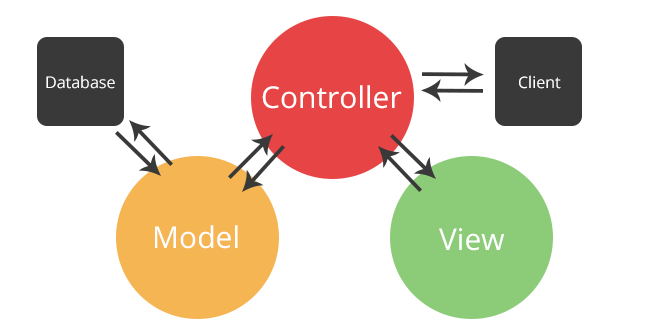
\includegraphics[width=\linewidth]{MVC}
    \caption{Arquitectura Modelo Vista-Controlador}
\end{figure}

El controlador es el elemento intermedio, el que comunica modelo y vista. Cualquier cambio
o interacción en la vista que requiera un cambio en el modelo, ya sea una petición \emph{GET}
o \emph{POST}, se hace a través del controlador.

Como nunca hay comunicación directa entre vistas y modelos (en ASP.NET Core), es el controlador
el que debe hacer las peticiones y cargas de los datos entre ambos.

Las acciones del usuario se controlan a través de JavaScript, que tiene diversos usos:
\begin{itemize}
 \item \textbf{\emph{JQuery}}: librería con funciones para su uso en JavaScript.
 \item \textbf{\emph{Ajax}}: permite hacer peticiones o consultas al controlador. Estas consultas pueden ser del tipo \emph{GET} (para obtener datos), o del tipo \emph{POST} (para enviar datos). Es la forma óptima de comunicación entre vista y controlador.
 \item \textbf{\emph{Datatables}}: librería de JavaScript que genera tablas de datos en base a
 los elementos que se pasan a través del modelo.
\end{itemize}

\subsection{Despliegue del servidor}
El despliegue del servidor es una de las fases más importantes del proyecto, ya que a través de este se podrá probar, experimentar y mostrar la funcionalidad del proyecto en su totalidad. 

Para hacer un despliegue, se han tenido en cuenta distintos métodos. Algunos de ellos eran inviables (por compatibilidad o entorno de desarrollo) y otros tenían un coste económico:
\begin{itemize}
 \item \textbf{Deployer}: herramienta que ayuda al despliegue de aplicaciones específicamente con PhP y a través de ssh.
 \item \textbf{Github Pages}: herramienta de despliegue de Github no compatible con el entorno de desarrollo utilizado.
 \item \textbf{MEAN}: opción para aplicaciones creadas a través de React.
 \item \textbf{LAMP}: distribuciones de Linux con Apache y MySql para PhP.
\end{itemize}

Otro gran problema es cómo alojar la base de datos de la aplicación, ya que se debería utilizar otra herramienta externa como Mongo Atlas, Postgresql, Azure, Google Cloud Platform...

La solución final ha sido utilizar el método que se utiliza en la empresa y en la mayoría de servidores locales, que es el IIS Express. Es una forma gratuita para desplegar aplicaciones web en un servidor de forma local. 

En este proyecto, se hará uso de los siguientes elementos:
\begin{itemize}
 \item \textbf{IIS Express}: herramienta para crear el servidor que apunta a la base de datos y a la carpeta web del proyecto.
 \item \textbf{SQL Server}: para la conexión de la base de datos.
 \item \textbf{SQL Management Studio}: para el gestor de la base de datos y su alojamiento. 
 \item \textbf{Directorio Web}: carpeta en la que se guardará el despliegue del proyecto web y al que apuntará el servidor.
\end{itemize}

Todo este montaje se hará dentro de una máquina virtual de Windows 10, que simulará un entorno local de un servidor web que funcionará a través de un navegador como por ejemplo Google Chrome. La aplicación se ejecuta en un puerto del localhost que se crea a través del despliegue.

\section{Dependencias y librerías}
\subsection{\emph{Bootstrap}}
\emph{Bootstrap}, como se ha explicado previamente en el apartado \ref{Conceptos Teóricos} de conceptos, es una librería que se utiliza como herramienta adicional a html. Contiene clases de estilos css y funciones de JavaScript.
\subsection{\emph{RotativaPDF}}
Es una librería que permite crear documentos a partir de vistas en html. En este caso particular, la mejor forma de utilizarla es importando la dependencia gracias al instalador de paquetes, configurando el archivo principal del programa, y finalmente utilizarla en los controladores.

Rotativa tiene una clase que devuelve un objeto en formato ``.pdf'', que se descarga automáticamente y se puede visualizar si se crea en una nueva ventana (esto se configura desde JavaScript). Además, el formato se puede configurar de distintas formas:
\begin{itemize}
\tightlist
 \item Orientación: vertical u horizontal.
 \item Tamaño: tanto de la letra como de la página (A3, A4...).
 \item Colores, formatos, textos. 
 \item Añadir pies de página, encabezados y más.
\end{itemize}
\subsection{\emph{Webfonts} y \emph{FontAwesome}}
Son archivos externos que permiten los iconos y formatos de texto para su uso en HTML, CSS y JavaScript.

\subsection{Otras Librerías}
A parte de las librerías indicadas anteriormente, hay que añadir las dependencias y ficheros internos para el desarrollo de los modelos en Core y los controladores, consultas, etc.
Entra ellas destacan:
\begin{itemize}
 \item \textbf{\emph{Serilog}}: herramienta de diagnóstico que crea los registros del programa. A través de esta herramienta, se crea una carpeta contenedora de los logs de la ejecución de la aplicación, que sobreescriben los archivos con errores, avisos, etc.
 \item \textbf{\emph{Microsoft.EntityFrameworkCore}}: librerías para el uso del contexto del modelo. Gracias a estas librerías se permite la conexión entre la base de datos y la propia aplicación, manipular modelos, consultas, etc. Entre las dependencias de \emph{EntityFramework}, destacan \emph{SqlServer}, \emph{Relational}...
 \item \textbf{Librerías de AspNetCore}: para el programa principal y otros usos, como las \emph{DataAnnotations} (para las clases de los modelos), MVC (para controladores). 
\end{itemize}

\section{Control de versiones}
La herramienta para el control de versiones utilizada ha sido Git, que es la más utilizada de forma global. Git permite la gestión y control del proyecto a través de una consola de comandos, con acciones como subir o bajar cambios, crear y cambiar ramas, listados de ramas o archivos, etc.

\section{Documentación}
La herramienta utilizada para toda la documentación del proyecto es LaTeX, con \href{https://overleaf.com/}{Overleaf}\footnote{Overleaf: https://overleaf.com/} como editor de textos.

Dentro de la documentación de este proyecto, podemos encontrar los siguientes elementos:
\begin{itemize}
 \item \textbf{Memoria}: documento principal del proyecto.
 \item \textbf{Anexos}: información que complementa a la memoria. 
 \item \textbf{Manual de usuario}: un manual de ayuda para el uso de la aplicación de cara al usuario. 
 \item \textbf{Manual de programador}: un manual de ayuda para la instalación y comprensión de la estructura del proyecto específico y orientado a desarrolladores.
 \item \textbf{Gestión del proyecto}: en él se detallan las fases (que son las milestones de GitHub) y los subprocesos que se han seguido a través del análisis y desarrollo.
 \item \textbf{Casos de uso}: pruebas de funcionalidad de los diferentes apartados de la aplicación.
 \item \textbf{Diagramas de clases}: relaciones entre los diferentes modelos que se usan en la aplicación.
\end{itemize}



\capitulo{5}{Aspectos relevantes del desarrollo del proyecto}


\section{Metodología de gestión del proyecto}
La metodología que se ha utilizado desde el principio ha sido la del modelo en cascada. La planificación que se realizó tomó este modelo para realizar cada una de las fases del proyecto de una forma lineal y efectiva.

Sin embargo, al poco tiempo del desarrollo fue necesario reconsiderar varias etapas, por lo que añadí el modelo de ruta crítica y así combinar ambos para tener una metodología consistente y que me permitiese hacer cambios sin romper la planificación inicial, o al menos aprovechando todos los recursos y el tiempo.

La aplicación de esta metodología resulta efectiva en los siguientes aspectos:
\begin{itemize}
 \item Reconfiguración de fases: al tener un modelo por el que estructurarlas (ruta crítica con prioridad temporal y necesidad de proceso), podía mover o cambiar cada fase en función de esto y el proyecto no se ve afectado.
 \item Economía del tiempo: la economía del tiempo se basa en aprovechar el tiempo que se necesita para realizar algo y así utilizar el restante para otras actividades o descanso. En este caso, con el modelo elegido que combina dos metodologías distintas, he podido aprovechar el tiempo para hacer las fases más prioritarias al principio, y, si sobraba tiempo, hacer el mayor número de mejoras posible.
 \item Cada una de las fases fue constante y proporcional en el tiempo, ajustándose bien a lo previsto inicialmente.
 \item Asegura que los procesos más necesarios se cumplen y dejar lo menos importante para el final hizo que se aprovechase bien el tiempo invertido y que ninguno de los requisitos funcionales quedase sin cubrir.
\end{itemize}

\section{Análisis de requisitos}
Los requisitos de software y arquitectura fueron bastante claros desde un principio, a excepción de algunas librerías extra que se han añadido a posteriori conforme se desarrollaba el proyecto y se modificaba o añadía alguna fase.

De esta forma, todas las herramientas que se utilizan han sido las mismas desde este análisis hasta el final del proyecto, solo añadiendo o cambiando algunas de ellas (cambios de versiones, añadidas librerías nuevas para el lado del cliente, etc.).

\section{Diseño de la base de datos}
La base de datos es una de las cosas que más ha ido cambiando desde que se diseñó al principio del proyecto, dada la necesidad de crear nuevas tablas en función de funcionalidades que al principio no se habían tenido en cuenta, o bien borrado y modificación de otras tablas que no se utilizaban o habían sido cambiadas en función de los cambios entre varias fases o etapas.

Esto se puede ver claramente en la carpeta de migraciones\footnote{Migraciones: https://github.com/ata1005/CSACVM/tree/master/CSACVM.AccesoDatos/Migrations} (\href{https://github.com/ata1005/CSACVM/tree/master/CSACVM.AccesoDatos/Migrations}{Migraciones - CSACVM}). En este directorio se guardan cada una de las migraciones que se han realizado en el proyecto con la base de datos. Cualquier cambio de tablas viene reflejado en esta carpeta.

\section{Iniciación del proyecto, dependencias y librerías}
En esta etapa ha ocurrido uno de los mayores problemas del desarrollo de la aplicación. Hay varias librerías y dependencias que no admitían ciertas versiones de otras, de modo que se ha tenido que cambiar la versión de éstas sobre la marcha.

Esto ha hecho que ciertos elementos de configuración del proyecto se modifiquen de forma brusca y han ocasionado uno de los mayores problemas: el fallo en la autodetección del configurador de la aplicación.

Este archivo era muy importante, dado que contiene la forma en la que trabaja el \emph{Serilog} (una de las librerías que fallaba por su versión) y la cadena de conexión con la base de datos. Al no detectar este archivo en el proyecto, no se podía obtener la cadena de conexión y por tanto la instancia de la base de datos no se creaba al iniciar el proyecto.

Este error se consiguió resolver rehaciendo la configuración de las dependencias de cada uno de los proyectos (AccesoDatos, Web, Modelos...) y cambiando de lugar el archivo. Al colocar el archivo en un lugar genérico del proyecto (un directorio superior), el proyecto era capaz de detectarlo y solucionar el problema. 

A partir de este punto, ninguna dependencia ha fallado, pero sí una librería: rotativa.
Rotativa es la librería que se encarga de la generación de ficheros. El problema de esta librería fue su configuración en el programa, ya que faltaba un directorio con los archivos de configuración necesarios para la ejecución de esta herramienta.

\section{Desarrollo principal del proyecto}
El desarrollo principal del proyecto conforma las etapas más importantes de la funcionalidad de la aplicación. Se han dividido los procesos en varias secciones ya que cada una de ellas ha tenido ciertas particularidades y aspectos relevantes en su desarrollo.

\subsection{Vistas de la página y diseño de interfaces}
Se ha seguido un diseño similar para la creación de las vistas de procesos específicos, como por ejemplo:
\begin{itemize}
 \item Vista de administración de usuarios y currículum.
 \item Vista con tablas de datos como currículum y notas.
\end{itemize}

La vista del inicio de sesión tiene un diseño muy similar a otras aplicaciones de CSA, que sigue el gradiente del fondo y como núcleo de la vista un elemento \emph{card} en su centro para poder iniciar sesión con el usuario.

La vista que más ha cambiado ha sido sin duda la página principal, ya que tenemos varios casos:
\begin{itemize}
 \item Si inicia sesión un administrador, verá los apartados de gestión principales (administración de usuarios y currículum) así como su propio perfil.
 \item Si inicia sesión cualquier otro usuario, verá su perfil, sus notas y la vista de currículos será distinta (solo podrá ver sus currículos).
\end{itemize}

Además, el diseño de esta interfaz se ha ido cambiando y adaptando en función de las fases del ciclo de vida que se han modificado, quitando o añadiendo botones, referencias y más.

\subsection{Configuración inicial de usuarios, inicios de sesión y registros}
Las primeras etapas del desarrollo, que han sido la configuración de usuarios, perfiles, inicio de sesión y registros, no han dado realmente muchos problemas. Los cambios más relevantes han sido tablas maestras para obtener ciertos datos en los perfiles de usuario, pero por lo demás no ha ocurrido nada relevante en su desarrollo.

\subsection{Currículum y exportación a formato ``.pdf''}
Esta ha sido una de las etapas que más ha cambiado, además de ser la más prioritaria y en la que más se ha invertido tiempo. 

Los cambios más visibles han sido:
\begin{itemize}
 \item Nuevas tablas en base de datos.
 \item Nuevos campos a varias tablas del modelo para aumentar los datos de los currículum
 \item Cambio en el diseño de la tabla de currículos para darle más funcionalidad.
 \item Cambio en el diseño de la exportación de los currículum (de un diseño propio al formato europeo estandarizado).
 \item Cambio en el diseño de la vista para editar currículum a medida que se añadían campos nuevos.
\end{itemize}

\subsection{Administración de currículos y usuarios}
Estas dos fases fueron añadidas posteriormente al análisis inicial y debido a la necesidad de realizarlas, se han colocado antes que otras en el modelo en cascada dada su prioridad.

A pesar del cambio entre fases, estas etapas no han llevado mucho tiempo y se han ajustado muy bien al desarrollo del modelo previsto, teniendo un solo diseño (no ha habido necesidad de modificarlo) y siendo ambas bastante parecidas.

El mayor cambio se verá a futuro a través de mejoras para añadir, por ejemplo, más filtros o campos.

\section{Cambios en las etapas del ciclo de vida}
A medida que se ha ido desarrollando el proyecto, las etapas o fases han ido cambiando en estructura y tamaño, añadiendo o quitando procesos y funcionalidades.

La mayoría de fases han recibido nuevos desarrollos para corregir errores o para añadir más funcionalidad de la que en un principio se había planificado. Sin embargo, uno de los cambios más relevantes ha sido el cambio de prioridad de procesos al añadir nuevas fases.

La fase de administración de usuarios y la de administración de currículos fueron añadidas a posteriori, tras ciertas reuniones de seguimiento con la empresa y su necesidad, ya que son unas funcionalidades que para ciertos equipos de la empresa pueden resultar muy útiles (sobre todo recursos humanos y administración).

Como ha sido necesario añadirlas, la distribución de fases se ha tenido que ajustar debido a la prioridad de estas nuevas etapas, de modo que otros procesos menos importantes se han dejado para más adelante o como mejoras a futuro (por ejemplo las publicaciones, el registro en el inicio de sesión, etc.).

\section{Despliegue del servidor web}
El despliegue del servidor web, por lo general, no ha dado tantos problemas como se esperaba en un principio. Para su creación, se genera una imagen del disco de Windows 10, se añade a la aplicación de VirtualBox y se configura y crea el entorno virtual.

La mayor complejidad viene cuando se crea el servidor de base de datos, que se realiza a través de SQL Server y no estaba muy familiarizado con ello.

La configuración del IIS Express no ha dado muchos problemas, el único error que se generaba para entrar en la aplicación, era solamente porque había que configurar usuarios de base de datos y darles permisos de lectura y escritura para la base de datos de la aplicación.

De esta forma, añadiendo el usuario a la cadena de conexión, la aplicación funcionaba perfectamente.
\capitulo{6}{Trabajos relacionados}

Hay varias aplicaciones dedicadas a la generación de currículos muy similares a lo que se quiere conseguir con este proyecto,

Una de ellas es, por ejemplo, el Curriculum Vitae Normalizado (CVN) del ministerio. Esta herramienta es el editor de currículos más completo y específico que podemos encontrar y tiene la ventaja de estar normalizado y estandarizado en lo que respecta a la mayoría de empresas y administraciones públicas. 

Al estar normalizado, forman la regla para la mayoría de los currículos que se necesitan en una empresa o una administración pública en España. La desventaja de este es, por ejemplo, que tiene una sobrecarga de datos y campos, muchos de ellos innecesarios, hasta el punto en que se puede hacer realmente tedioso completarlo, más aún a la hora de rellenar un documento para uso genérico. 

Además de esto, esta herramienta se enfoca mucho en la información y experiencia académica y no tanto en lo laboral.

También tenemos un editor más pequeño y más visual, como es \href{https://www.cvmaker.es/}{\mbox{CV Maker}}\footnote{CV Maker Online: https://www.cvmaker.es/}, que comprende los campos principales de un currículum, bastante similar a las características de este proyecto en cuanto a sencillez y objetivos.

Sin embargo, la necesidad de realizar este proyecto, viene dada por las siguientes ventajas:
\begin{itemize}
 \item Se necesita un gestor interno y común para la empresa, para que sus usuarios (trabajadores) tengan un currículum con un formato similar en cuanto a estructura y datos.
 \item Es muy útil para la empresa al tener formatos únicos de los currículos y por los que poder filtrar a través de distintos campos.
 \item Es una herramienta sencilla de instalar y mantener con el tiempo, así como para desarrollar nuevas funciones y utilidades a futuro.
 \item El hardware y software utilizado es idéntico al resto de proyectos de la empresa, por lo que es muy fácil integrarlo con los demás.
\end{itemize}

\capitulo{7}{Conclusiones y Líneas de trabajo futuras}

En esta última sección de la memoria se expondrán tanto las conclusiones extraídas a raíz de la finalización del proyecto, como las conclusiones de análisis de futuras mejoras o cosas que podrían cambiarse de la aplicación.

\section{Conclusiones}

En cuanto a las conclusiones que podemos extraer, se destacan:

\begin{itemize}
\item
  La aplicación cumple el objetivo inicial en cuanto a sencillez, comodidad y efectividad.
  Los usuarios tanto de la empresa como nuevos trabajadores podrán dejar y mantener su currículum actualizado y los administradores y trabajadores de recursos humanos podrán explotar la información de forma interna y utilizar la herramienta para los fines que se deseen.
\item
  El desarrollo del proyecto con las herramientas utilizadas ha sido una decisión acertada, ya que no solo es una de las formas más efectivas para desarrollar este tipo de aplicaciones, sino que además el haberla utilizado previamente ha hecho que, en muchos casos, evite caer en ciertos errores y esto se vea afectado negativamente en el tiempo del desarrollo.
\item
  Gracias a este proyecto en el que se utilizan todo tipo de librerías, dependencias y herramientas, he logrado no solo profundizar en aquellas que ya conocía de antes, sino además descubrir nuevas formas de desarrollo y competencias a raíz de metodologías que con las que no estaba familiarizado. En este sentido también destaco crear el entorno virtual por mí mismo y dotarlo de todo lo necesario para hacer un despliegue correcto.
\item
  La metodología que se ha aplicado me ha ayudado tanto a evitar fallos de forma temprana como a reducir el tiempo de desarrollo de muchas tareas, ya que, como se ha explicado en el cuarto apartado, consigo priorizar las fases en tiempo y en necesidad de desarrollo.
\end{itemize}

\section{Líneas de trabajo futuras}

La entrega de este proyecto de fin de grado no marca el punto y final de la aplicación, sino el primer despliegue de la versión oficial de producción en la empresa, que es al final el objetivo principal que se tenía con ella.

A pesar de ser la versión oficial y final de este trabajo, el proyecto se ampliará y estará sujeto a muchos cambios y mejoras que ya se plantean:

\begin{itemize}
\item  En el repositorio del proyecto, se encuentran algunas de las mejoras planteadas para el        desarrollo a futuro de la aplicación, como viene a ser actualizaciones de diseño, nuevas 
  pantallas, atributos de una red social, adición de nuevas funcionalidades similares a la gestión de currículos, poder unir la aplicación con otras internas de la empresa, etc.
\item
  En cuanto a la gestión de currículum, se prevee que a medida que se vaya utilizando, salgan nuevos campos por los que poder filtrar la información, la posibilidad de descargar varios archivos de golpe, añadir nuevos campos para rellenar los currículos, etc.
\end{itemize}


\nocite{*}
\bibliographystyle{plain}
\bibliography{bibliografia}

\end{document}
